\setchapterpreamble[u]{\margintoc}
\chapter{Conclusions and Future Work}\label{chapter-conclusions-and-future-work}

The core question the research aims to consider is:
\begin{quote}
  \emph{How can applying analytics improve software development and software testing for mobile apps in practice?}~\href{overall-research-question}{Research Question, repeated here}\index{Research questions}.
\end{quote}

\subsection{Research questions lead to six perspectives}~\label{rq-leads-to-six-perspectives}
The six perspectives are illustrated in Figure~\ref{fig:six-perspectives-in-the-research-questions-section}~\sidenote{Source figure:~\href{https://docs.google.com/drawings/d/1SafKu3uqgl-s8-I8iWSSWmFY4NdlNpw8v6ZiJDGh50c/edit?usp=sharing}{Google Docs: Six Perspectives drawing}.} and paraphrased below:
{\footnotesize
\begin{enumerate}
    %\setlength\itemsep{-0.5em} %\itemsep0em
    \item [1a] What do app developers say they do? (understand the \emph{status quo} from their perspective).\index{Research questions}
    \item [2a] What's possible in terms of improving their processes, their practices?
    \item [1b] What does their source code (and other available development artefacts) tell us about their use of mobile analytics? (understand current behaviours in terms of the code that's implemented)~\sidenote{NB: it might be useful to reanalyse the projects we studies to identify which ones actively include crash reporting.}.
    \item [2b] What's possible in terms of improving the product (and particularly the mobile app) through the application/use of mobile analytics?
    \item [3a] What do we learn about various current mobile analytics tools?
    \item [3b] What improvements are possible for mobile analytics tools based on what was learned in the various case studies?
\end{enumerate}
}

\section{Conclusions}
When developers apply mobile analytics to find failures they are able to significantly improve the stability/reliability of their mobile app. When they stop paying attention and don't apply mobile analytics entropy returns eventually for a variety of reasons including new releases of the operating system, updates to third-party software used by the app, such as the Android System WebView, and flaws in ongoing software development and maintenance of the app. The developers do not need to address all the issues that are reported to effect material improvements (and indeed some issues are impractical for developers to fix in the time and resources they have available).

When developers choose to include in-app mobile analytics they generally prefer to use those mobile analytics as their primary source of information, even if the platform analytics also finds a common subset of the same failures. The meta-data collected and reported by the in-app mobile analytics combined with the availability of reports even at low usage volumes of the app are key drivers in this preference to use the in-app mobile analytics reporting. For two of the app-centric case studies the data collected by in-app mobile analytics \Glspl{sdk} was sufficient that they chose not to use in-app mobile analytics in their apps. Some projects choose to have several in-app \Glspl{sdk} embedded in their apps, often for distinct purposes.

There appears to be a general, perhaps misplaced, trust that the mobile analytics tools are accurate - both by the app developers and in the literature. Eighteen distinct flaws were found in the mobile analytics services, and there are probably many more flaws waiting to be discovered given the practical limitations placed by both industrial collaboration and the scope of a PhD. 

The field of mobile analytics evolved throughout the research period and it is likely to continue to evolve for years to come. The reporting and analysis appears to be fairly perfunctory and there may be significant scope to improve the analysis and reporting.

The human motivations that determine the use of mobile analytics are at least as interesting as the quantitative results of the effects of whatever use occurs. With the exception of the \myindex{Moonpig} development team, none of the teams used mobile analytics on an ongoing, proactive basis. 


\clearpage
\section{Future Work}
Future work incorporates future research work and areas for practitioners including app developers and tool developers.

\begin{figure}
    \centering
    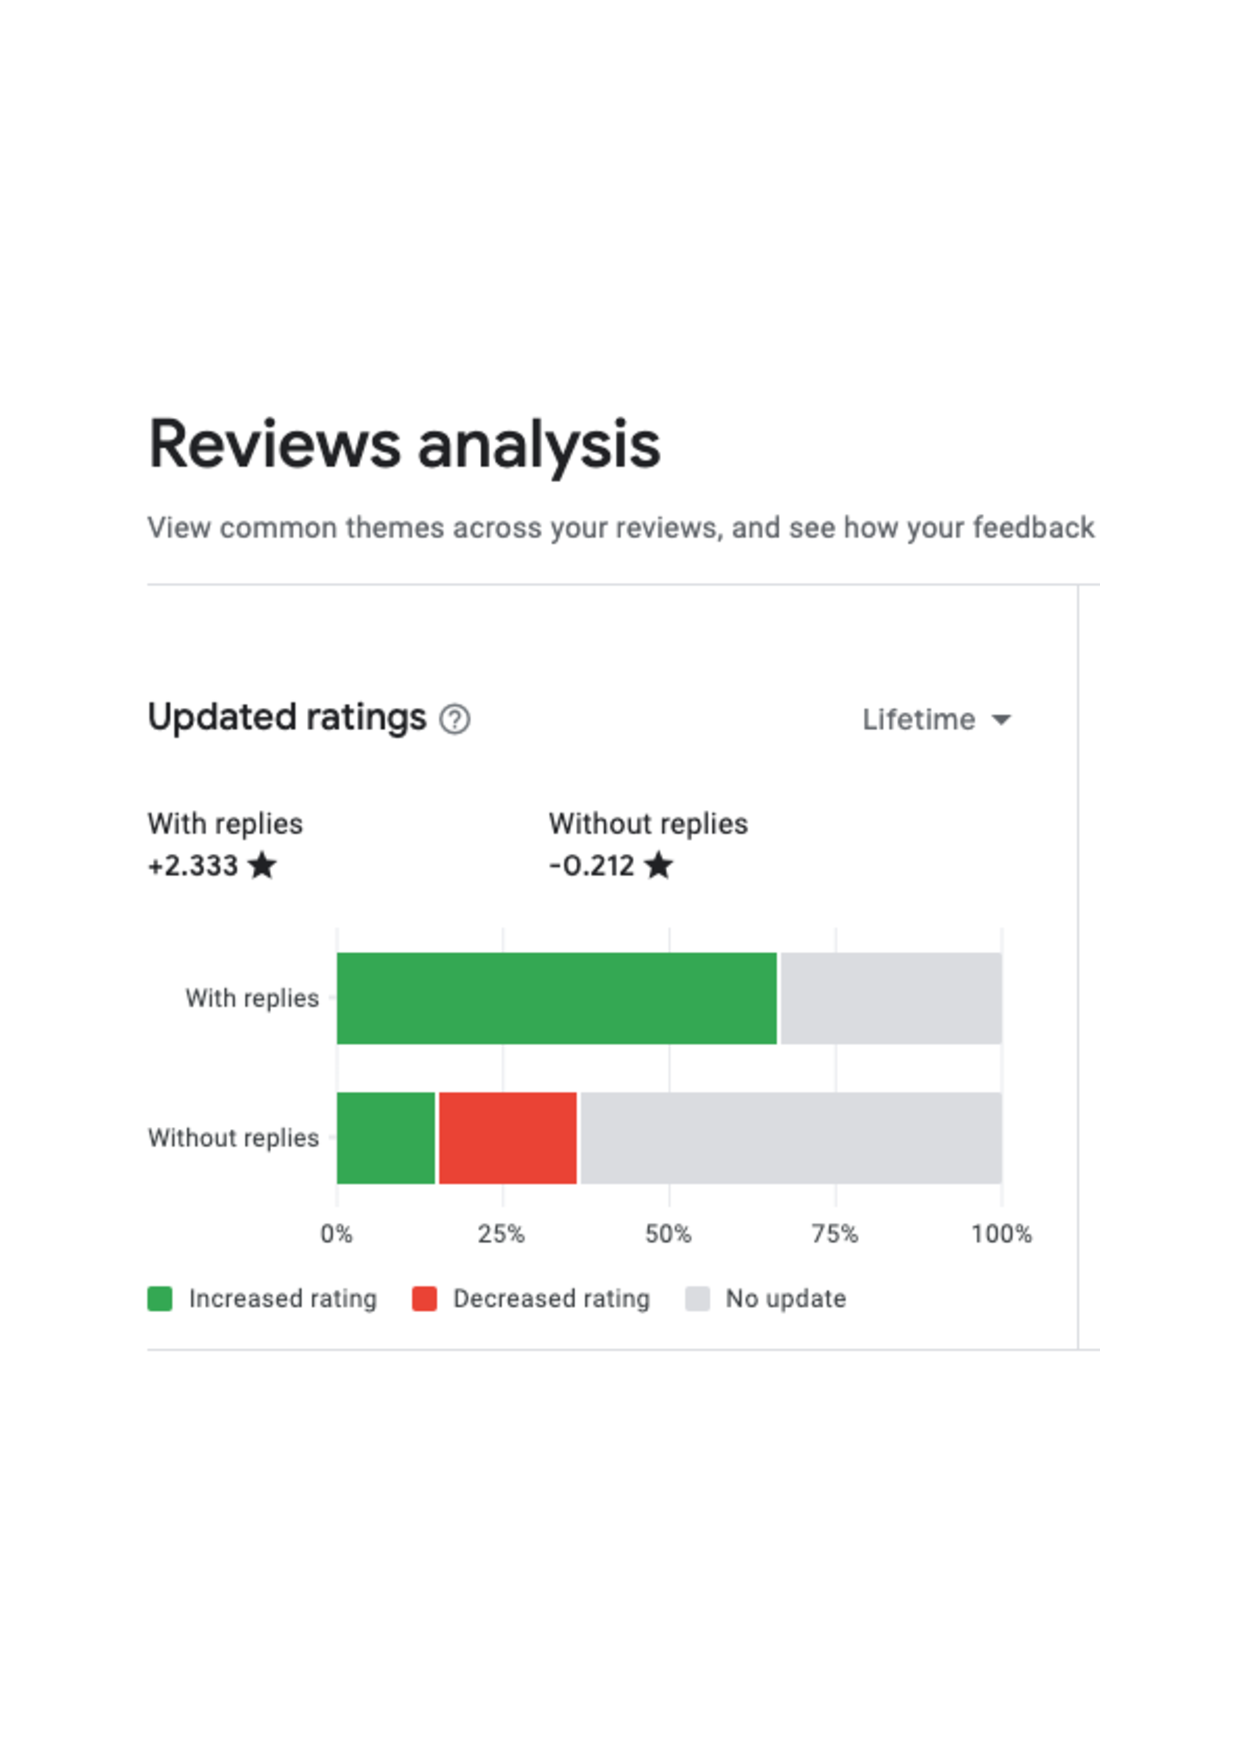
\includegraphics[width=\linewidth]{images/google-play-console/PhET-Review-Analysis-Screenshot-2022-09-07.pdf}
    \caption{Example of Review Analysis in Google Play Console for the Physics and Chemistry simulations app}
    \label{fig:PhET-Review-Analysis-Screenshot-2022-09-07}
\end{figure}

\begin{figure}
    \centering
    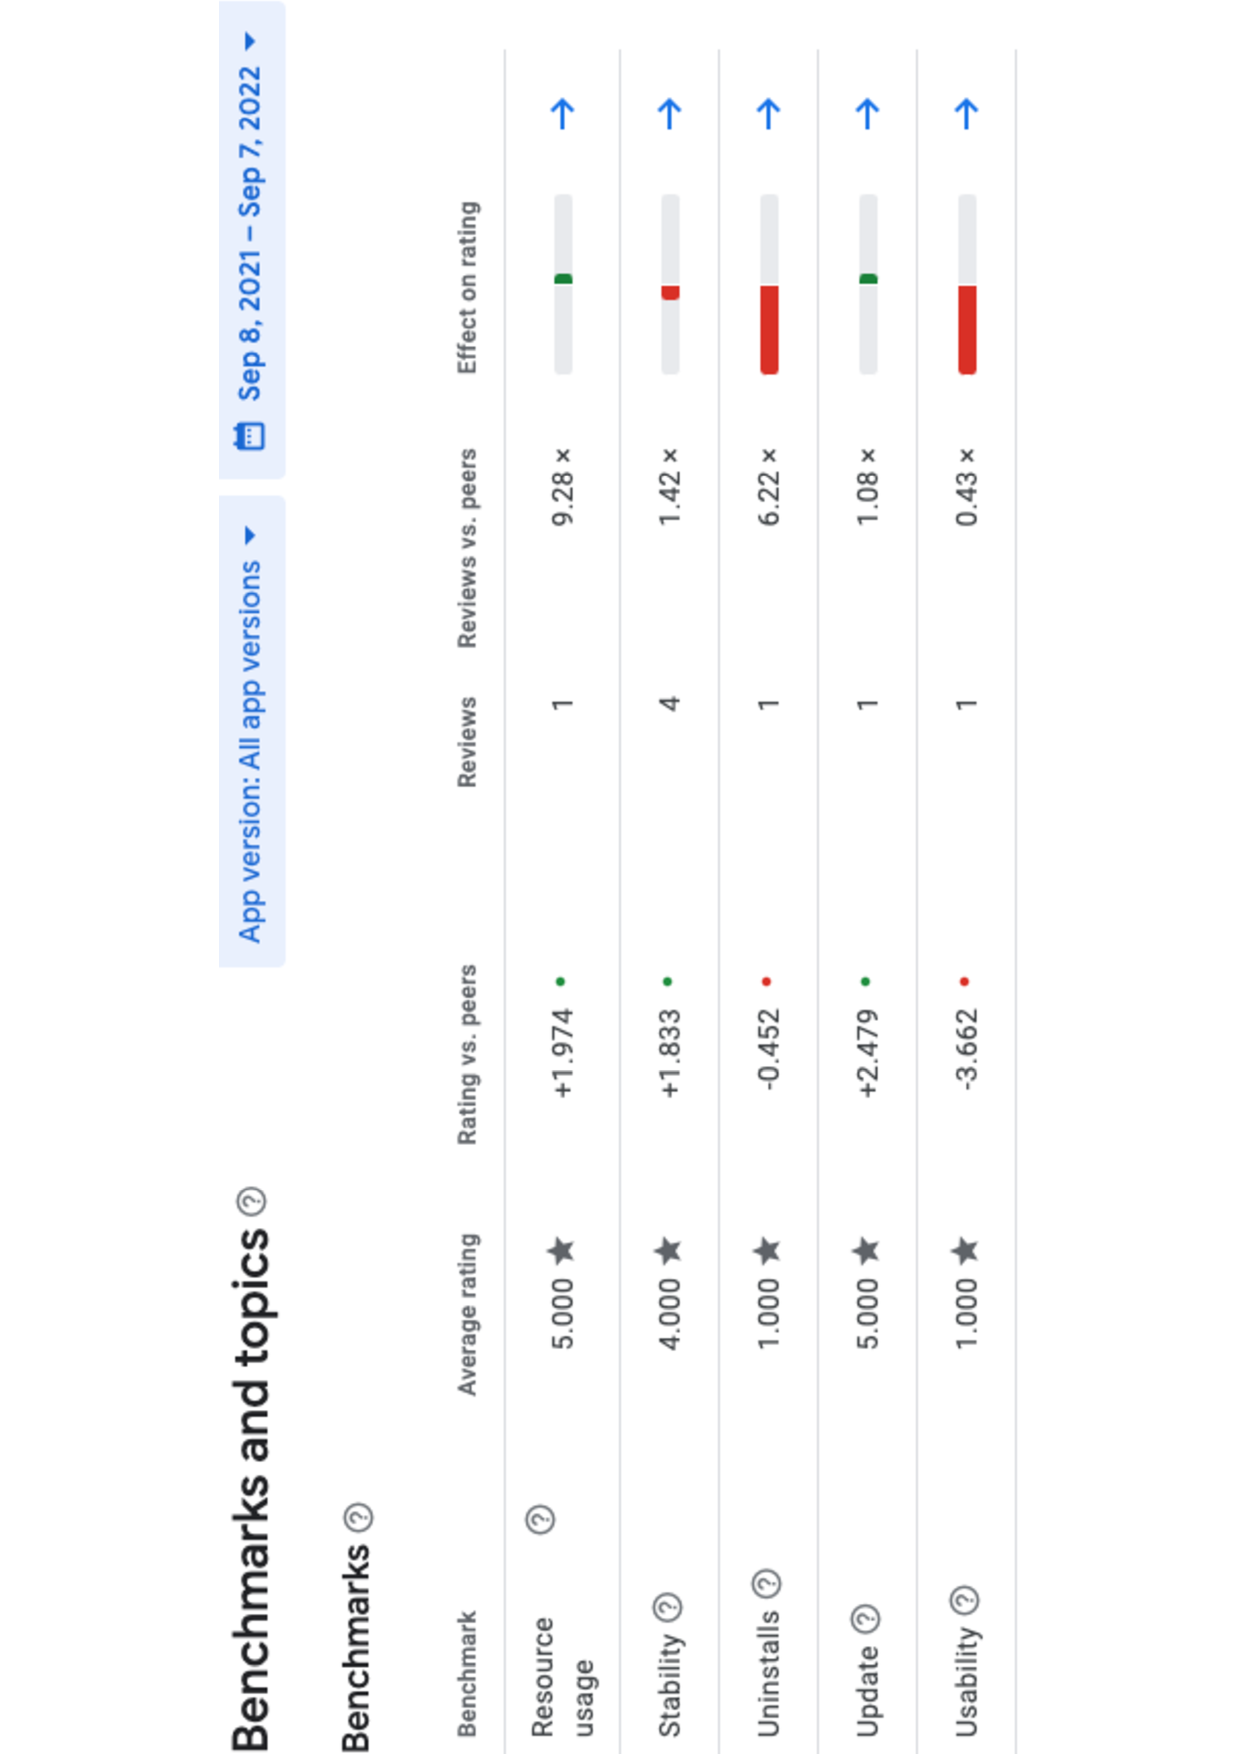
\includegraphics[width=\linewidth]{images/google-play-console/PhET-Review-Benchmarks-Screenshot-2022-09-07.pdf}
    \caption{Example for the \Gls{phet} app of Benchmarks provided automatically by Google Play Console}
    \label{fig:PhET-Review-Benchmarks-Screenshot-2022-09-07}
\end{figure}

\subsection{Combining human- and mobile analytics feedback}~\label{fw-combining-reviews-and-mobile-analytics-topic}
In \secref{aiu-discussion-section} the concept of symbiotic information sources was discussed, for example to investigate any intersections and gaps between what users report in terms of bugs and crashes, \emph{etc.} and what mobile analytics reports. Android app developers have good access to both platform analytics, via \myindex{Android Vitals}, and various online Review Analysis tools, illustrated in Figures \ref{fig:PhET-Review-Analysis-Screenshot-2022-09-07} and \ref{fig:PhET-Review-Benchmarks-Screenshot-2022-09-07}, to the best of my knowledge there has not been material research either into the Review Analysis tools, nor into any symbiosis between the reviews, review analysis, or mobile analytics. Such research may provide insights into the review analysis (which may have its own flaws and characteristics) and the extent to which mobile analytics and reviews provide actionable information to developers, \emph{etc.}


\subsection{Investigation of additional app ecosystems}~\label{fw-investigate-additional-ecosystems}
If the mobile app ecosystem influences other ecosystems such as desktop app ecosystems\index{Desktop app ecosystem}, as claimed in the opening section of \secref{chapter-related-work}, perhaps this research will also apply to those app ecosystems, albeit there are likely to be many distinctions as each ecosystem is distinct and unique.  What are the engineering challenges and realities in those app ecosystems, what sort of analytics do those platforms provide? and what do the apps use? To what extent can the app developers rely on analytics to learn of instabilities or failures in their apps, and can they apply similar techniques to those described in this research? 

Closer to home, there has been little study of mobile analytics in regional app stores, such as those in China~\sidecite{wang2018_beyond_google_play}.


